% =====================================================================
% WitnessRAG: desenho da proposta, versão 3 (versão de leitura)
% Compilar: latexmk -pdf witnessrag-proposta-v3.tex
%
% Mesmo método da versão 2, explicado com texto, exemplos e figuras.
% Só ficam as fórmulas necessárias para entender o método. As definições
% formais e as provas estão em witnessrag-proposta-v2.tex.
% =====================================================================
\documentclass[11pt]{article}
\usepackage[margin=2.4cm]{geometry}
\usepackage[T1]{fontenc}
\usepackage[utf8]{inputenc}
\usepackage[brazilian, provide=*]{babel}
\usepackage{amsmath,amssymb}
\usepackage{booktabs,tabularx,array}
\usepackage{enumitem}
\usepackage{xcolor}
\usepackage{pifont}
\usepackage{float}
\usepackage{tikz}
\usetikzlibrary{arrows.meta,positioning,fit,backgrounds,calc,shapes.geometric}
\usepackage[numbers]{natbib}
\usepackage[hidelinks]{hyperref}

\newcommand{\op}[1]{\textsc{#1}}
\newcommand{\rel}[1]{\textsf{#1}}
\newcommand{\inc}[1]{\textsf{?#1}}
\newcolumntype{Y}{>{\raggedright\arraybackslash}X}
\setlength{\parskip}{3pt}

\title{\textbf{WitnessRAG}\\[4pt]
\large Memória que responde com provas}
\author{}
\date{Desenho da proposta, versão 3 (versão de leitura)}

\begin{document}
\maketitle

\begin{abstract}
\noindent
Um agente de linguagem com memória longa precisa, a cada pergunta, escolher
poucos trechos do histórico para ler. A busca por similaridade escolhe trechos
parecidos com a pergunta, mas não sabe dizer se eles bastam para responder. O
WitnessRAG procura uma \emph{prova} da resposta. A memória guarda a conversa
de duas formas: como trechos de texto e como um grafo de fatos, todos datados.
Para cada pergunta, o sistema busca evidências, escreve um plano de busca a
partir delas e segue o plano pelo grafo até encontrar uma \emph{testemunha}:
os poucos fatos dos quais a resposta decorre. Encontrar a testemunha é o sinal
de parada. O contexto entregue ao leitor contém a testemunha e, no espaço que
sobra, os trechos mais relevantes.
\end{abstract}

% =====================================================================
\section{O problema e a ideia}

\paragraph{O problema.} A memória de um agente conversacional acumula meses
de diálogo. Para responder a uma pergunta, o agente não pode ler tudo:
um recuperador escolhe alguns trechos (cinco, nos nossos experimentos) e um
leitor responde a partir deles. O recuperador mais comum escolhe os trechos
mais parecidos com a pergunta. Isso funciona quando a resposta está em um
único trecho que usa as mesmas palavras da pergunta, e falha em três
situações frequentes:
\begin{itemize}[leftmargin=*,itemsep=2pt]
\item \textbf{A resposta está espalhada.} ``Onde Melanie já acampou?'' tem
  três respostas, ditas em três sessões diferentes. Os cinco trechos mais
  parecidos podem trazer duas.
\item \textbf{A resposta exige um encadeamento.} Em ``Onde mora a irmã de
  Ana?'', o trecho que diz ``Bia se mudou para Recife'' não menciona Ana. Ele
  só é relevante depois que se sabe que Bia é a irmã.
\item \textbf{A resposta depende de datas.} Em ``Quando Melanie acampou em
  junho?'', o trecho certo é o de junho, mas trechos de julho sobre acampamento
  são igualmente parecidos com a pergunta.
\end{itemize}
Nos três casos a causa é a mesma: a similaridade mede o quanto um trecho se
parece com a pergunta, e não se o conjunto escolhido é \emph{suficiente}
para respondê-la.

\paragraph{A ideia: procurar uma prova.} Em bancos de dados, a prova de que
um resultado está correto é o conjunto mínimo de registros que o produz,
chamado de \emph{testemunha}~\citep{buneman2001why,green2007provenance}.
Levamos esse conceito para a memória de agentes: a testemunha de uma resposta
é o menor conjunto de fatos da memória do qual ela decorre. Para ``Onde mora a
irmã de Ana?'', a testemunha são dois fatos, ``Bia é irmã de Ana'' e ``Bia
mora em Recife''. A testemunha tem dois usos no método:
\begin{enumerate}[leftmargin=*,itemsep=2pt]
\item \textbf{Saber quando parar.} Enquanto não há testemunha, a busca
  continua; quando há, a busca pode parar.
\item \textbf{Saber o que o contexto precisa conter.} Os trechos de onde vêm
  os fatos da testemunha entram obrigatoriamente no contexto do leitor.
\end{enumerate}

\paragraph{Três decisões de desenho.} O resto do método decorre de três
escolhas:
\begin{enumerate}[leftmargin=*,itemsep=2pt]
\item \textbf{A memória tem duas camadas e um tempo.} A conversa é guardada
  como trechos de texto, que o leitor lê, e como um grafo de fatos, em que a
  prova é procurada. Todo trecho e todo fato têm data.
\item \textbf{Toda pergunta recebe um plano.} Até a pergunta mais simples vira
  um plano de busca. Datas e expressões como ``mais recente'' fazem parte do
  plano.
\item \textbf{Uma única pontuação guia toda a busca.} A mesma fórmula ordena
  trechos e fatos, combinando similaridade, importância e proximidade no
  tempo. O plano decide quanto vale cada parte.
\end{enumerate}

% =====================================================================
\section{Visão geral do processo}
\label{sec:visao}

O método tem duas fases (Figura~\ref{fig:fluxo}). A primeira acontece uma
vez, antes das perguntas: \op{Registrar} transforma a conversa em memória. A
segunda acontece a cada pergunta: um ciclo de quatro passos procura a prova,
e \op{Responder} entrega o resultado ao leitor.

\begin{figure}[H]
\centering
\resizebox{\textwidth}{!}{%
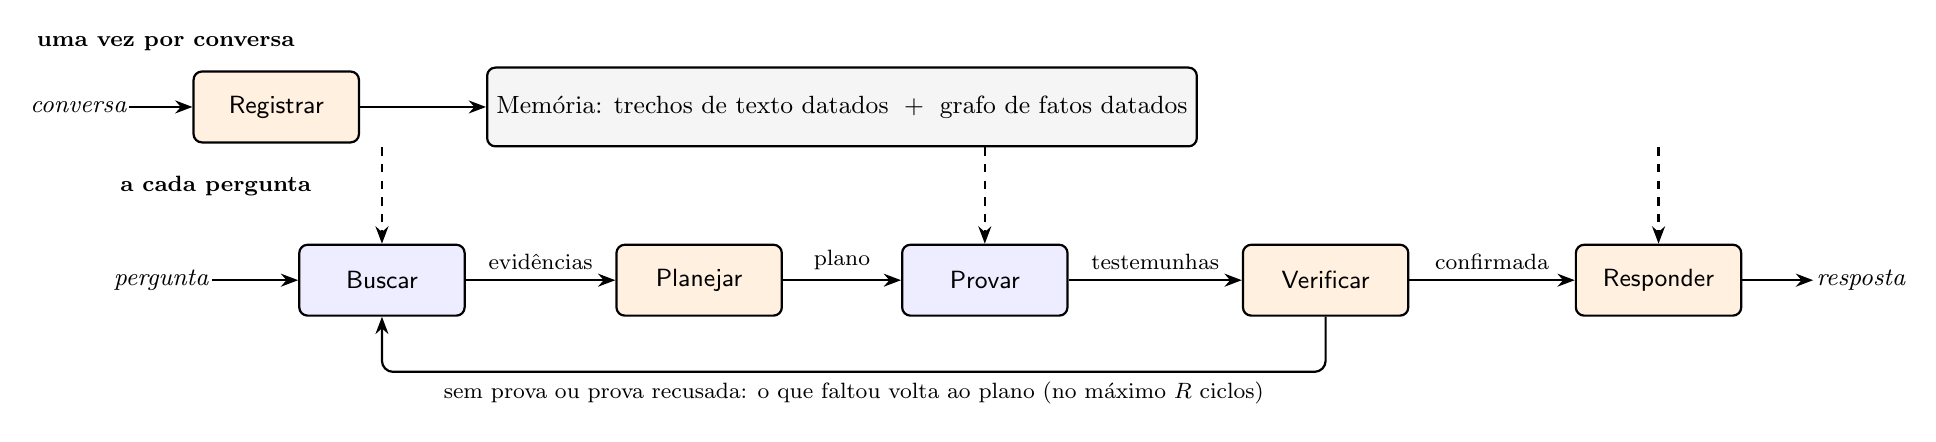
\begin{tikzpicture}[
  verb/.style={draw, rounded corners=3pt, thick, fill=blue!7, minimum
    height=9mm, minimum width=21mm, font=\sffamily\small},
  llm/.style={verb, fill=orange!12},
  obj/.style={font=\small\itshape, inner sep=1pt},
  arr/.style={-{Stealth[length=2.2mm]}, thick},
  lab/.style={font=\footnotesize, midway, above},
]
\node[obj] (q) at (0,0) {pergunta};
\node[verb, right=11mm of q] (bus) {Buscar};
\node[llm, right=19mm of bus] (pla) {Planejar};
\node[verb, right=15mm of pla] (pro) {Provar};
\node[llm, right=22mm of pro] (ver) {Verificar};
\node[llm, right=21mm of ver] (res) {Responder};
\node[obj, right=9mm of res] (a) {resposta};
\draw[arr] (q) -- (bus);
\draw[arr] (bus) -- node[lab]{evidências} (pla);
\draw[arr] (pla) -- node[lab]{plano} (pro);
\draw[arr] (pro) -- node[lab]{testemunhas} (ver);
\draw[arr] (ver) -- node[lab]{confirmada} (res);
\draw[arr] (res) -- (a);
\draw[arr, rounded corners=4pt] (ver.south) -- ++(0,-7mm) -| node[pos=0.25, below,
  font=\footnotesize]{sem prova ou prova recusada: o que faltou volta ao plano (no máximo $R$ ciclos)} (bus.south);
\node[draw, thick, rounded corners=3pt, fill=gray!8, minimum height=10mm,
  align=center, font=\small] (mem) at ($(pla)!0.5!(pro)+(0,2.2)$)
  {Memória: trechos de texto datados \;+\; grafo de fatos datados};
\node[llm, left=16mm of mem] (reg) {Registrar};
\node[obj, left=8mm of reg] (h) {conversa};
\draw[arr] (h) -- (reg);
\draw[arr] (reg) -- (mem);
\draw[arr, dashed] (mem.south -| bus) -- (bus.north);
\draw[arr, dashed] (mem.south -| pro) -- (pro.north);
\draw[arr, dashed] (mem.south -| res) -- (res.north);
\node[font=\footnotesize\bfseries, anchor=west] at ($(h.west)+(0,0.8)$) {uma vez por conversa};
\node[font=\footnotesize\bfseries, anchor=west] at ($(q.west)+(0,1.2)$) {a cada pergunta};
\end{tikzpicture}}
\caption{Fluxo do WitnessRAG. Componentes em laranja chamam o modelo de
linguagem; em azul, não. Linhas tracejadas indicam leitura da memória.}
\label{fig:fluxo}
\end{figure}

\paragraph{Um exemplo do começo ao fim.} Considere a pergunta ``Onde Melanie
já acampou?'' sobre uma conversa do LoCoMo~\citep{maharana2024locomo}. A
resposta correta é ``praia, montanhas e floresta'', ditas em três sessões
(27/6, 6/7 e 15/7 de 2023).
\begin{enumerate}[leftmargin=*,itemsep=3pt]
\setcounter{enumi}{-1}
\item \textbf{Registrar} (antes das perguntas). Cada sessão da conversa vira
  trechos de texto. De cada trecho, o modelo extrai fatos curtos, como
  \rel{acampou\_em}(Melanie, montanhas), com a data em que o acampamento
  aconteceu. Os fatos formam um grafo: Melanie é um nó, montanhas é outro, e o
  fato é a aresta entre eles.
\item \textbf{Buscar.} O sistema pega os trechos mais relevantes para a
  pergunta. Nesta primeira busca ainda não há plano, e a relevância é dominada
  pela similaridade. Suponha que vieram os trechos com as sessões de 27/6 e
  6/7, mas não o trecho com a sessão de 15/7.
\item \textbf{Planejar.} O modelo lê a pergunta \emph{e esses trechos} e
  escreve o plano: procurar arestas \rel{acampou\_em} saindo de Melanie, com
  o destino desconhecido, \rel{acampou\_em}(Melanie, \inc{onde}). Como a
  pergunta pede todos os lugares, o plano marca a resposta como um conjunto.
\item \textbf{Provar.} O sistema segue o plano no grafo. Encontra três
  arestas que casam com o padrão: montanhas, praia e floresta. Cada uma é uma
  testemunha de um fato só. A da floresta veio de um trecho que a busca
  inicial não trouxe.
\item \textbf{Verificar.} O modelo lê as três testemunhas com suas datas e
  confirma que respondem à pergunta. O ciclo termina.
\item \textbf{Responder.} O contexto recebe os trechos das três testemunhas
  e completa as vagas restantes com os trechos mais relevantes. O leitor
  responde ``praia, montanhas e floresta''.
\end{enumerate}

Se no passo 3 não houvesse testemunha, ou se no passo 4 o modelo recusasse a
prova, o sistema registraria o que faltou (por exemplo, ``nenhuma aresta
parecida com \rel{acampou\_em}'') e voltaria ao passo 1 para um novo ciclo,
com um plano corrigido.

\paragraph{Vocabulário.} A Tabela~\ref{tab:vocab} resume os termos usados no
resto do texto.

\begin{table}[H]
\centering
\small
\begin{tabularx}{\textwidth}{@{}l Y Y@{}}
\toprule
Termo & O que é & Exemplo \\
\midrule
Trecho & bloco contíguo da conversa (até 2048 tokens), com as datas das sessões que cobre & o trecho com as sessões de 9/6 a 3/7/2023 \\
Fato & relação entre duas coisas, com data e trecho de origem & \rel{acampou\_em}(Melanie, montanhas), 19--25/6/2023 \\
Grafo & os fatos vistos como arestas entre entidades & Melanie $\to$ montanhas \\
Evidências & trechos trazidos pela busca, usados para planejar & os trechos com as sessões de 27/6 e 6/7 \\
Plano & o padrão de fatos a procurar, mais período e pesos & \rel{acampou\_em}(Melanie, \inc{onde}) \\
Testemunha & fatos da memória que encaixam no plano inteiro & o fato das montanhas \\
Contexto & os trechos entregues ao leitor & os trechos das testemunhas e outros relevantes \\
\bottomrule
\end{tabularx}
\caption{Termos principais.}
\label{tab:vocab}
\end{table}

% =====================================================================
\section{Como a memória é construída}
\label{sec:registrar}

\op{Registrar} roda uma vez por conversa e produz as duas camadas da memória.
A Figura~\ref{fig:grafo} mostra o caminho de três falas reais até o grafo.

\begin{figure}[H]
\centering
\resizebox{\textwidth}{!}{%
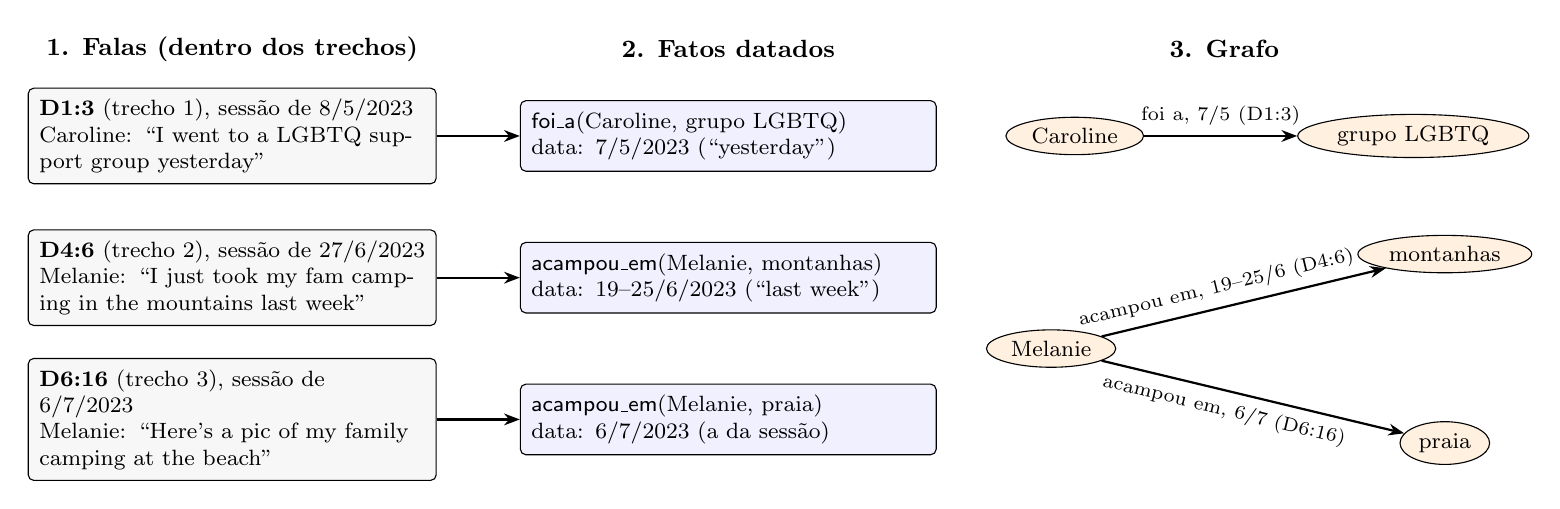
\begin{tikzpicture}[
  txt/.style={draw, rounded corners=2pt, fill=gray!6, text width=4.9cm,
    font=\footnotesize, align=left, inner sep=4pt},
  fact/.style={draw, rounded corners=2pt, fill=blue!6, text width=5.0cm,
    font=\footnotesize, align=left, inner sep=4pt},
  ent/.style={draw, ellipse, fill=orange!12, font=\footnotesize, inner sep=2pt},
  arr/.style={-{Stealth[length=2mm]}, thick},
  head/.style={font=\small\bfseries},
]
\node[head] at (0,1.1) {1. Falas (dentro dos trechos)};
\node[head] at (6.3,1.1) {2. Fatos datados};
\node[head] at (12.6,1.1) {3. Grafo};
\node[txt] (t1) at (0,0) {\textbf{D1:3} (trecho 1), sessão de 8/5/2023\\ Caroline: ``I went to a LGBTQ support group yesterday''};
\node[txt] (t4) at (0,-1.8) {\textbf{D4:6} (trecho 2), sessão de 27/6/2023\\ Melanie: ``I just took my fam camping in the mountains last week''};
\node[txt] (t6) at (0,-3.6) {\textbf{D6:16} (trecho 3), sessão de 6/7/2023\\ Melanie: ``Here's a pic of my family camping at the beach''};
\node[fact] (f1) at (6.3,0) {\rel{foi\_a}(Caroline, grupo LGBTQ)\\ data: 7/5/2023 (``yesterday'')};
\node[fact] (f4) at (6.3,-1.8) {\rel{acampou\_em}(Melanie, montanhas)\\ data: 19--25/6/2023 (``last week'')};
\node[fact] (f6) at (6.3,-3.6) {\rel{acampou\_em}(Melanie, praia)\\ data: 6/7/2023 (a da sessão)};
\draw[arr] (t1) -- (f1);
\draw[arr] (t4) -- (f4);
\draw[arr] (t6) -- (f6);
\node[ent] (car) at (10.7,0) {Caroline};
\node[ent] (grp) at (15.0,0) {grupo LGBTQ};
\node[ent] (mel) at (10.4,-2.7) {Melanie};
\node[ent] (mon) at (15.4,-1.5) {montanhas};
\node[ent] (pra) at (15.4,-3.9) {praia};
\draw[arr] (car) -- node[above, font=\scriptsize]{foi a, 7/5 (D1:3)} (grp);
\draw[arr] (mel) -- node[pos=0.42, above, sloped, font=\scriptsize]{acampou em, 19--25/6 (D4:6)} (mon);
\draw[arr] (mel) -- node[pos=0.42, below, sloped, font=\scriptsize]{acampou em, 6/7 (D6:16)} (pra);
\end{tikzpicture}}
\caption{Da conversa ao grafo, com falas reais do LoCoMo. O modelo extrai
fatos de cada trecho e resolve expressões de tempo pela data da sessão da fala.
Nomes iguais viram o mesmo nó, e cada aresta guarda a fala de onde veio.}
\label{fig:grafo}
\end{figure}

\paragraph{1. Trechos.} A conversa é cortada em blocos de até 2048 tokens,
sem partir falas ao meio. Um trecho pode cobrir mais de uma sessão; cada fala
guarda a data da sua sessão, e o trecho guarda o intervalo dessas datas.
Os trechos são a camada que o leitor lê no final.

\paragraph{2. Fatos.} Um modelo de linguagem lê o texto em janelas curtas e
escreve os fatos que encontra, no formato (sujeito, relação, objeto). O
vocabulário das relações é livre: o extrator usa o verbo que o texto usa
(``acampou em'', ``foi a'', ``se mudou para''). Não há uma lista fixa de
relações. Por isso, mais adiante, a busca compara relações por
\emph{similaridade de significado}, e não por igualdade de texto.

\paragraph{3. Entidades.} Nomes que se referem à mesma coisa (``Mel'' e
``Melanie'') são unidos em uma única entidade. Cada entidade é um nó do
grafo, e cada fato é uma aresta entre dois nós.

\paragraph{4. Datas.} Cada fato recebe a data em que o evento
\emph{aconteceu}, que nem sempre é a data em que foi dito. Expressões
relativas são resolvidas a partir da data da sessão: ``yesterday'', dito em
8/5/2023, vira 7/5/2023; ``last week'', dito em 27/6/2023, vira a semana de
19 a 25/6. Quando a fala não tem expressão de tempo, o fato recebe a data da
sessão. Toda data é guardada como um intervalo de dias: um dia, uma semana ou
um mês.

\paragraph{5. Importância.} Cada fala recebe uma nota de importância entre 0
e 1, que mede o quanto o falante marcou o evento como significativo, pela
intensidade emocional do texto~\citep{flexa2026bridging,mcgaugh2004amygdala}.
O fato herda a nota da fala de onde veio. A nota é calculada uma vez e não
depende da pergunta.

\subsection*{Do que a memória é feita}

Ao fim do \op{Registrar}, a memória tem quatro tipos de elemento, ligados entre
si (Tabela~\ref{tab:anatomia}). Um fato é mais do que a tripla sujeito,
relação e objeto: ele carrega também \emph{quando} o evento aconteceu,
\emph{quão importante} ele foi para quem falou e \emph{de onde} veio, até a fala
exata. São esses campos extras que permitem buscar por data, preferir o que foi
marcante e mostrar ao leitor e ao verificador o texto original.

\begin{table}[H]
\centering
\small
\begin{tabularx}{\textwidth}{@{}l Y Y@{}}
\toprule
Elemento & Campos & Exemplo \\
\midrule
Fala & identificador; falante; texto; data da sessão & D4:6; Melanie; ``I just took my fam camping in the mountains last week''; 27/6/2023 \\
Trecho & identificador; as falas que contém, em ordem; intervalo das datas das suas sessões; importância média das falas & trecho 2; falas D3:11 a D5:12; 9/6 a 3/7/2023 \\
Entidade (nó) & nome canônico; variantes do nome que foram unidas & Melanie (``Mel'') \\
Fato (aresta) & sujeito (entidade); relação (predicado em texto livre); objeto (entidade ou valor); data do evento (intervalo de dias); importância; trecho e fala de origem & (Melanie, acampou em, montanhas); 19--25/6/2023; 0,68; trecho 2, D4:6 \\
\bottomrule
\end{tabularx}
\caption{Anatomia da memória. As arestas são dirigidas (do sujeito para o
objeto) e o grafo pode ter várias arestas entre os mesmos nós, por exemplo
quando o mesmo fato é contado em sessões diferentes, cada uma com sua data e
sua origem.}
\label{tab:anatomia}
\end{table}

Três observações ajudam a ler a tabela. Primeiro, a relação não vem de uma
lista fixa: é o verbo que o texto usou, e a busca compara relações por
significado. Segundo, a data do fato é a do \emph{evento}, resolvida a partir da
data da fala; a data da sessão continua disponível na fala. Terceiro, a memória
não guarda resumos nem rótulos de categoria de pergunta: tudo nela vem da
conversa.

\paragraph{O resultado.} A memória fica com duas camadas ligadas entre si.
Na camada de texto estão as falas e os trechos, com data. Na camada lógica está
o grafo: nós são entidades e arestas são fatos. As camadas têm papéis
diferentes. O grafo serve para \emph{raciocinar}: seguir de Ana para a irmã e da
irmã para a cidade. O texto serve para \emph{ler}: o leitor recebe as falas
originais, com todo o contexto que um fato resumido perde. A ligação entre as
duas (cada fato aponta para a sua fala) é o que permite passar de uma prova no
grafo para os trechos que o leitor precisa ver.

% =====================================================================
\section{Como procuramos na memória}
\label{sec:busca}

\subsection{Uma pontuação para toda a busca}
\label{sec:pontuacao}

Toda decisão de ordem no método, tanto na escolha de trechos quanto nos passos
dentro do grafo, usa a mesma pontuação, com três sinais entre 0 e 1:
\begin{itemize}[leftmargin=*,itemsep=2pt]
\item \textbf{Similaridade}: o quanto o item se parece com o que se procura.
  Para um trecho, a comparação é com a pergunta, combinando busca por
  significado (embeddings) e por palavras. Para um fato, a comparação é com o
  passo do plano: a relação é parecida e os nomes batem?
\item \textbf{Importância}: a nota gravada na construção da memória.
\item \textbf{Proximidade no tempo}: o quanto a data do item está perto do
  \emph{período de referência} do plano.
\end{itemize}
A pontuação é a soma ponderada dos três:
\begin{equation}
\label{eq:pontuacao}
\boxed{\;\text{pontuação}(x)=w_{\text{sim}}\cdot\text{sim}(x)
+w_{\text{imp}}\cdot\text{imp}(x)+w_{\text{tempo}}\cdot\text{prox}(x)\;}
\end{equation}
Os pesos somam 1 e são escolhidos pelo plano, em três níveis por sinal
(nenhum, normal, forte). A similaridade nunca fica com menos da metade, o que
garante que um item sem relação com a pergunta nunca passa à frente de um item
muito relacionado só por ser importante ou recente.

Os valores dos níveis foram calibrados sem LLM, sobre as dez conversas do
LoCoMo, medindo se a evidência anotada entra nos cinco trechos
(\texttt{docs/prova-v3-offline.md}). Com o período ``hoje'', dar peso ao
tempo ou à importância mudou de 12\% a 72\% dos contextos sem aumentar essa
revocação. Por isso, no nível normal, todo o peso fica na similaridade, e o
contexto é o mesmo da busca híbrida. Quando a pergunta cita uma data, peso
0,3 no tempo elevou a revocação em todas as categorias; esse é o nível forte
do tempo. A importância forte recebe 0,1. É o planejador quem liga o nível
forte, quando a pergunta tem data, ``primeira vez'', ``mais recente'' ou algo
marcante.

\paragraph{Recência é proximidade a uma data.} A proximidade no tempo usa uma
única fórmula:
\begin{equation}
\label{eq:prox}
\text{prox}(x)=\exp\!\Big(-\frac{\text{dias entre a data de } x \text{ e o período de referência}}{\lambda}\Big).
\end{equation}
Dentro do período, a distância é zero e a proximidade é 1; fora dele, ela
cai aos poucos. A escala $\lambda$ define a velocidade da queda: para um
período citado na pergunta, é metade da sua largura (no mínimo uma semana);
para o presente ou o início da conversa, é uma fração da duração da conversa.
A mesma fórmula cobre as três buscas temporais que aparecem em perguntas:
\begin{itemize}[leftmargin=*,itemsep=1pt]
\item \textbf{Período = hoje}: favorece o mais novo. É a recência comum,
  usada por padrão.
\item \textbf{Período = início da conversa}: favorece o mais antigo, para
  ``qual foi a primeira vez''.
\item \textbf{Período = uma data citada} (``em junho''): favorece o que
  aconteceu naquela data, com uma recência medida em relação a junho, e não
  ao presente.
\end{itemize}

\paragraph{Exemplo: ``Quando Melanie acampou em junho?''} O plano usa junho
de 2023 como período e dá peso forte ao tempo, $(0{,}7;\;0;\;0{,}3)$. Há quatro
fatos de acampamento na memória, todos igualmente parecidos com a pergunta:
\begin{center}
\small
\begin{tabular}{@{}l l c c c@{}}
\toprule
Fato & Data do evento & Distância & prox & $0{,}3\cdot$prox \\
\midrule
montanhas & 19--25/6 (``last week'', dito em 27/6) & 0 dias & 1,00 & 0,30 \\
praia & 6/7 & 6 dias & 0,67 & 0,20 \\
sem lugar & 8--9/7 (``two weekends ago'', dito em 17/7) & 8 dias & 0,59 & 0,18 \\
floresta & 15/7 & 15 dias & 0,37 & 0,11 \\
\bottomrule
\end{tabular}
\end{center}
Com $\lambda=15$ dias (metade de junho), o acampamento de junho vence, e a
resposta é ``na semana antes de 27 de junho'', que é a resposta correta. A
data funciona como preferência, e não como filtro rígido: um fato fora do
período perde pontos, mas não some. Isso protege contra erros na resolução
das datas.

\subsection{Buscar evidências}

\op{Buscar} pega os $m$ trechos (20, por padrão) com maior pontuação e os
junta às evidências. Na primeira busca, o plano ainda não existe, e usa-se o
plano padrão: sem padrão de fatos, período ``hoje'' e pesos padrão. Nos ciclos
seguintes, a busca usa o plano do ciclo anterior, que pode trazer outro
período ou outros pesos e, com eles, outros trechos. As evidências só
crescem. Elas servem para planejar e para procurar a prova primeiro no lugar
certo, e não são ainda o contexto final.

\subsection{Planejar}

\op{Planejar} é uma chamada ao modelo de linguagem. Ele recebe a pergunta, as
evidências (com datas e os fatos que elas contêm) e, a partir do segundo
ciclo, o que faltou no ciclo anterior. Ele devolve um plano com quatro
partes:
\begin{enumerate}[leftmargin=*,itemsep=1pt]
\item \textbf{O padrão de fatos a procurar}, escrito como uma sequência de
  passos. Cada passo é uma aresta procurada, com nomes conhecidos e incógnitas
  (marcadas com \textsf{?}). Passos ligados por uma incógnita formam um
  caminho.
\item \textbf{O tipo de resposta}: um valor ou um conjunto.
\item \textbf{O período de referência}: hoje, por padrão, ou a data citada.
\item \textbf{Os pesos} da pontuação.
\end{enumerate}

Planejar \emph{depois} de buscar resolve três problemas. O planejador escreve
as relações com as palavras que aparecem na memória, e não com as da
pergunta. Ele resolve as expressões de tempo da pergunta usando as datas que
vê. E ele ajusta os pesos conforme o que as evidências mostram.

\begin{table}[H]
\centering
\small
\begin{tabularx}{\textwidth}{@{}Y l Y@{}}
\toprule
Pergunta & Padrão de fatos & Resto do plano \\
\midrule
Qual é a identidade de Caroline? & \rel{identidade}(Caroline, \inc{x}) & valor \\
Quando Caroline foi ao grupo de apoio? & \rel{foi\_a}(Caroline, grupo de apoio, \inc{quando}) & valor; a data é a incógnita \\
Onde Melanie já acampou? & \rel{acampou\_em}(Melanie, \inc{onde}) & conjunto \\
Quando Melanie acampou em junho? & \rel{acampou\_em}(Melanie, \inc{}, \inc{quando}) & valor; período junho/2023; tempo com peso alto \\
Qual foi a viagem mais recente de Jon? & \rel{viajou\_para}(Jon, \inc{x}) & valor; período hoje; tempo com peso alto \\
Onde mora a irmã de Ana? & \rel{irmã\_de}(\inc{y}, Ana) $\to$ \rel{mora\_em}(\inc{y}, \inc{z}) & valor; dois passos ligados por \inc{y} \\
\bottomrule
\end{tabularx}
\caption{Exemplos de planos. Perguntas simples têm um passo só. Em perguntas
``quando'', a data do fato é a incógnita. Um \textsf{?} sozinho indica que o
valor daquela ponta não importa.}
\label{tab:planos}
\end{table}

\subsection{Provar: procurar a prova no grafo}
\label{sec:provar}

\op{Provar} segue o plano pelo grafo, sem chamar o modelo de linguagem. A
Figura~\ref{fig:busca} mostra o processo para ``Onde mora a irmã de Ana?'',
cujo plano tem dois passos: \rel{irmã\_de}(\inc{y}, Ana) e depois
\rel{mora\_em}(\inc{y}, \inc{z}).

\begin{figure}[H]
\centering
\resizebox{0.8\textwidth}{!}{%
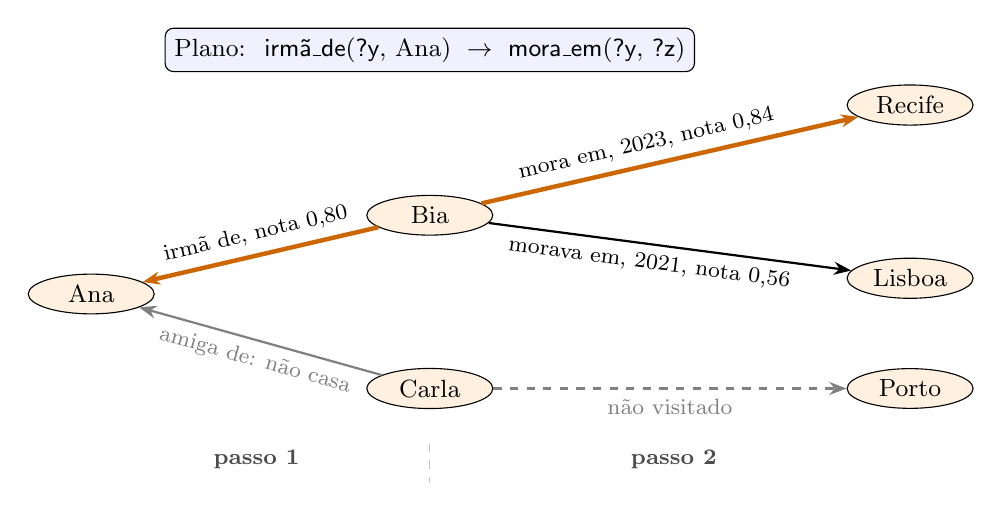
\begin{tikzpicture}[
  ent/.style={draw, ellipse, fill=orange!12, font=\small, inner sep=2pt, minimum width=16mm},
  arr/.style={-{Stealth[length=2.2mm]}, thick},
  win/.style={arr, draw=orange!80!black, line width=1.6pt},
  lab/.style={font=\footnotesize, midway},
]
\node[draw, rounded corners=3pt, fill=blue!6, font=\small, align=center] at (4.3,3.1)
  {Plano:\; \rel{irmã\_de}(\inc{y}, Ana) \;$\to$\; \rel{mora\_em}(\inc{y}, \inc{z})};
\node[ent] (ana) at (0,0) {Ana};
\node[ent] (bia) at (4.3,1.0) {Bia};
\node[ent] (car) at (4.3,-1.2) {Carla};
\node[ent] (rec) at (10.4,2.4) {Recife};
\node[ent] (lis) at (10.4,0.2) {Lisboa};
\node[ent] (por) at (10.4,-1.2) {Porto};
\draw[win] (bia) -- node[lab, above, sloped]{irmã de, nota 0,80} (ana);
\draw[arr, gray] (car) -- node[lab, below, sloped]{amiga de: não casa} (ana);
\draw[win] (bia) -- node[lab, above, sloped, pos=0.45]{mora em, 2023, nota 0,84} (rec);
\draw[arr] (bia) -- node[lab, below, sloped, pos=0.45]{morava em, 2021, nota 0,56} (lis);
\draw[arr, gray, dashed] (car) -- node[lab, below]{não visitado} (por);
\node[font=\footnotesize\bfseries, gray!60!black] at (2.1,-2.1) {passo 1};
\node[font=\footnotesize\bfseries, gray!60!black] at (7.4,-2.1) {passo 2};
\draw[gray!50, dashed] (4.3,-1.9) -- (4.3,-2.4);
\end{tikzpicture}}
\caption{Procurando a prova de ``Onde mora a irmã de Ana?''. Passo 1: a
partir de Ana, só arestas parecidas com ``irmã de'' são aceitas, e
\inc{y} = Bia. Passo 2: a partir de Bia, as arestas parecidas com ``mora em''
são candidatas; com os pesos padrão, o fato mais recente tem nota maior. O
caminho em laranja é a testemunha, e a resposta é \inc{z} = Recife. As notas
são ilustrativas.}
\label{fig:busca}
\end{figure}

A busca funciona assim:
\begin{enumerate}[leftmargin=*,itemsep=2pt]
\item \textbf{Começar pelo que se sabe.} O primeiro passo é o que tem mais
  nomes conhecidos. Aqui, \rel{irmã\_de}(\inc{y}, Ana): Ana é conhecida. O
  nome ``Ana'' é ligado ao nó correspondente do grafo por similaridade de
  nome.
\item \textbf{Aceitar só arestas que casam.} Das arestas ligadas a Ana, só
  entram as que têm relação parecida com ``irmã de'', acima de um limiar de
  similaridade. ``Amiga de'' não passa.
\item \textbf{Fixar as incógnitas.} Cada aresta aceita dá um valor para as
  incógnitas do passo: \inc{y} = Bia.
\item \textbf{Andar para o próximo passo.} O passo seguinte usa o valor
  fixado: \rel{mora\_em}(Bia, \inc{z}). As candidatas são as arestas de Bia
  parecidas com ``mora em'': Recife (2023) e Lisboa (2021). Uma incógnita
  que aparece em dois passos tem de receber o mesmo valor nos dois.
\item \textbf{Dar nota a cada passo.} Cada aresta usada recebe a pontuação
  da Eq.~\eqref{eq:pontuacao}, com os pesos do plano, e o caminho recebe a
  média geométrica das notas dos seus passos. Assim, similaridade, importância e tempo
  pesam em cada passo da exploração, e não só no fim. Para não explodir, a
  busca guarda a cada passo só os melhores caminhos parciais (algumas
  centenas).
\item \textbf{Reconhecer a prova.} Um caminho que cobre todos os passos do
  plano é uma testemunha. A resposta é o valor da incógnita pedida:
  \inc{z} = Recife. Para mudar o contexto, a prova precisa ser seletiva:
  poucas respostas (até 3), poucas combinações de fatos (até 3), busca sem
  cortes e casamento acima de um limiar. O limiar vale sobre o casamento com
  os passos do plano, não sobre a pontuação: os pesos do plano decidem qual
  prova é preferida, não se uma prova vale.
\end{enumerate}

\paragraph{Primeiro nas evidências, depois no grafo inteiro.} A prova é
procurada primeiro só entre os fatos que vêm dos trechos de evidência. Uma
prova ali é a mais segura, porque o planejador leu esses trechos ao escrever
o plano. Só quando não há prova nas evidências a busca se estende ao grafo
inteiro. Para respostas do tipo conjunto, a busca no grafo inteiro sempre
acontece, porque não dá para saber se um conjunto está completo olhando só
parte da memória. Foi o que trouxe a floresta no exemplo da
Seção~\ref{sec:visao}.

\paragraph{Quando não há prova.} Se nenhum caminho completo é encontrado,
\op{Provar} devolve a \emph{lacuna}: os passos do plano que não tiveram
nenhuma aresta aceita, ou o passo em que todos os caminhos morreram. A lacuna
diz ao planejador exatamente o que corrigir.

\subsection{Verificar: parar ou continuar}

\op{Verificar} é o único componente que encerra o ciclo. Se não há
testemunha, ele devolve ``continuar'' sem chamar o modelo de linguagem. Se a
prova já está nos trechos do contexto, não há o que confirmar: o ciclo
termina sem chamada, porque a prova não mudaria nada. Se a prova mudaria o
contexto, uma chamada lê as testemunhas como frases datadas, cada uma com a
fala de onde veio (falante, data da sessão e falas vizinhas), e confirma cada
resposta, a menos que a prova não responda à pergunta (entidade, período ou
tipo errados, ou falta de suporte). Nesse caso o motivo da recusa entra na
lacuna.

Assim, o critério de parada é: \emph{existe uma testemunha e ela foi
confirmada}. A verificação confirma; ela não procura nada. Quando o ciclo
continua, a nova busca usa o plano atual e o planejador escreve um plano
novo que ataca a causa da lacuna: trocar o nome da relação, corrigir um nome
próprio, mudar o período ou os pesos. O ciclo roda no máximo $R$ vezes (2,
por padrão). O papel lembra a autorreflexão do
Reflexion~\citep{shinn2023reflexion}, com uma diferença: aqui a lacuna é
objetiva (qual passo falhou ou por que a prova foi recusada), e não um
diagnóstico livre.

\paragraph{O caso mais comum é o mais barato.} Para ``When did Caroline go to
the LGBTQ support group?'', a primeira busca já traz o trecho da sessão de
8/5/2023, em que Caroline diz ``I went to a LGBTQ support group yesterday''.
O fato \rel{foi\_a}(Caroline, grupo LGBTQ), com data 7/5/2023, está nas
evidências, e o plano \rel{foi\_a}(Caroline, grupo LGBTQ, \inc{quando}) se
completa sem sair delas. O verificador confirma, e o leitor responde ``7 May
2023''. Como o trecho da prova já está no contexto, são duas chamadas ao
modelo: planejar e ler.

\subsection{Responder: montar o contexto}

O contexto tem $k$ vagas (5, por padrão) e é montado em duas etapas:
\begin{enumerate}[leftmargin=*,itemsep=1pt]
\item Entram os trechos de onde vêm os fatos das testemunhas confirmadas: uma
  testemunha para respostas do tipo valor e quantas couberem para conjuntos.
\item As vagas restantes ficam com os trechos de maior pontuação em toda a
  memória, sob o plano final.
\end{enumerate}
Em símbolos, com $D(W)$ para os trechos de origem da testemunha $W$:
\begin{equation}
\label{eq:contexto}
\text{contexto}=D(W)\;\cup\;\text{os } k-|D(W)| \text{ melhores trechos restantes}.
\end{equation}
Esse é o contexto de maior pontuação entre os que contêm a prova:
\emph{relevância sob restrição de prova}. Para limitar o risco de uma prova
errada, as testemunhas podem trazer no máximo $k_W$ trechos que não estariam
entre os $k$ melhores, e os primeiros $k-k_W$ trechos nunca saem: $k_W=2$ para
um plano composto (vários fatos ligados, ou uma resposta do tipo conjunto) e
$k_W=1$ para um plano de um fato e um valor. Se não houve prova confirmada, o
contexto é simplesmente o dos $k$ melhores trechos. Hipóteses sem prova, como
as sondas de concordância do controlador anterior, não mudam o contexto: no
teste sem LLM elas trocaram quase metade dos contextos de perguntas simples e
reduziram a revocação.

O leitor recebe os trechos com suas datas, os da testemunha por último, mais
perto da pergunta. A testemunha já aponta a resposta; o leitor dá a forma
final e faz contas com datas quando a pergunta pede (``quanto tempo
depois\ldots'').

% =====================================================================
\section{O que o desenho garante e quanto custa}

\begin{itemize}[leftmargin=*,itemsep=3pt]
\item \textbf{A prova chega ao leitor.} Quando há testemunha confirmada,
  todos os fatos dela, com suas datas, estão em trechos do contexto.
\item \textbf{A prova muda pouco o contexto.} Em relação ao contexto que se
  teria sem prova, no máximo $k_W$ trechos são trocados. Um erro de prova
  custa no máximo duas vagas.
\item \textbf{A busca por similaridade é um caso particular.} Com todo o peso
  na similaridade e sem prova, o método devolve exatamente os $k$ trechos mais
  similares. Cada ablação do método é, portanto, uma variação controlada de
  uma linha de base conhecida.
\item \textbf{Custo.} Cada ciclo faz uma chamada para planejar e, se a prova
  mudaria o contexto, uma para verificar; a leitura é mais uma. O total vai de
  2 chamadas, quando o primeiro ciclo termina com a prova já no contexto, a 5,
  com $R=2$. Buscar e provar não usam o modelo. A construção da memória roda
  uma vez por conversa.
\end{itemize}

% =====================================================================
\section{Desenho experimental}

\paragraph{Protocolo.} Seguimos o protocolo do GAM~\citep{yan2025gam}. A
avaliação principal é o LoCoMo, com F1 e BLEU-1 por categoria em 1.540
perguntas, sem as adversariais. Completam a avaliação o HotpotQA com 56K,
224K e 448K tokens~\citep{yang2018hotpotqa}, o RULER
128K~\citep{hsieh2024ruler} e o NarrativeQA~\citep{kocisky2018narrativeqa}.
Leitor, modelo de embeddings~\citep{chen2024bgem3}, tamanho de trecho (2048
tokens) e número de trechos no contexto (5) são os mesmos para todos os
métodos.

\paragraph{Linhas de base.} Recuperação híbrida (embeddings e palavras, com
RRF~\citep{cormack2009rrf}), GraphRAG~\citep{edge2024graphrag}, HippoRAG
2~\citep{gutierrez2025hipporag2}, GAM, Zero-Mem e um executor de consultas
sobre os \emph{mesmos} fatos, sem o critério de testemunha. Este último separa
o ganho da prova do ganho da extração de fatos.

\paragraph{Perguntas de pesquisa.}
\begin{enumerate}[label=\textbf{Q\arabic*},leftmargin=*,itemsep=1pt]
\item \emph{A prova como critério.} Escolher o contexto exigindo a prova
  melhora a resposta em relação às linhas de base, em cada categoria?
\item \emph{Planejar depois de buscar.} Um plano escrito com as evidências é
  melhor do que um plano escrito só com a pergunta?
\item \emph{Pesos escolhidos pelo plano.} Pesos definidos pelo planejador
  superam pesos fixos? Qual é o efeito da importância e do tempo, em especial
  nas perguntas temporais?
\item \emph{Parada e custo.} Com que frequência a prova já está nas
  evidências iniciais? Quantas chamadas e tokens o método gasta por pergunta,
  comparado ao GAM?
\end{enumerate}

\begin{table}[H]
\centering
\small
\begin{tabularx}{\textwidth}{@{}l Y l@{}}
\toprule
Variante & O que muda & Pergunta \\
\midrule
Similaridade pura & todo o peso na similaridade, sem plano nem prova & base \\
Sem prova & plano e pesos, mas o contexto nunca exige testemunha & Q1 \\
Plano cego & o planejador vê só a pergunta & Q2 \\
Pesos fixos & sempre os pesos padrão & Q3 \\
Sem importância / sem tempo & peso zero para um dos sinais & Q3 \\
Sem evidências primeiro & a prova é sempre procurada no grafo inteiro & Q4 \\
Verificação fundida & verificar e ler na mesma chamada & Q4 \\
\bottomrule
\end{tabularx}
\caption{Ablações. Cada linha muda uma única decisão do método.}
\label{tab:ablacoes}
\end{table}

% =====================================================================
\appendix
\section{Implementação}

{\sloppy O desenho está implementado como a opção \texttt{-{}-proof-controller}. O
controlador fica no método \texttt{\_retrieve\_proof} do arquivo
\texttt{wrag/\allowbreak methods/\allowbreak witnessrag.py}. Os
controladores anteriores, \texttt{selective-v1} e \texttt{agnostic-v1},
continuam disponíveis para comparação. A versão formal, com definições e
provas, está em \texttt{witnessrag-proposta-v2.tex}.\par}

\begin{table}[H]
\centering
\small
\begin{tabularx}{\textwidth}{@{}l Y@{}}
\toprule
Componente & Onde e como \\
\midrule
\op{Registrar} & \texttt{wrag/witness/dated\_memory.py}: data do evento de todo fato (expressão relativa resolvida pela data da fala; sem expressão, a data da sessão), importância pela ativação emocional da fala, fala de origem de cada fato \\
Pontuação & \texttt{wrag/witness/scoring.py}: níveis de peso, período (hoje, início, janela), proximidade $\exp(-\text{dias}/\lambda)$ \\
\op{Buscar} & ordena todos os trechos pela pontuação do plano; sem peso de tempo e importância, é exatamente a ordem da busca híbrida \\
\op{Planejar} & \texttt{wrag/witness/plan.py}: uma chamada que vê a pergunta, o vocabulário e até 30 fatos datados das evidências; devolve consulta (com espaço de tempo para ``quando''), agregação, período e níveis de peso; saída inválida vira plano inválido \\
\op{Provar} & \texttt{wrag/witness/search.py}: a junção soma importância e tempo ao casamento de cada passo; variável de tempo liga a data do fato; primeiro os fatos das evidências, depois o grafo inteiro \\
\op{Verificar} & \texttt{wrag/witness/confirm.py}: decisão por resposta candidata, com a fala de origem de cada fato; só é chamada quando a prova mudaria o contexto \\
\op{Responder} & prova confirmada entra pela cauda ($k_W=2$ composto, 1 simples); mesmo conjunto de trechos que o híbrido preserva a ordem do híbrido \\
\bottomrule
\end{tabularx}
\caption{Onde cada componente está no código.}
\label{tab:mapa}
\end{table}

\paragraph{Valores usados.} Trechos de 2048 tokens; $k=5$; $m=20$ trechos por
busca; $k_W=2$ (composto) e 1 (simples); 400 caminhos guardados por passo;
limiar de similaridade de relação 0,65; até 3 respostas e 3 combinações de
fatos numa prova; casamento mínimo 0,45; $\lambda$ mínimo de 7 dias e um
quarto da duração da conversa para ``hoje'' e ``início''; $R=2$ ciclos; nível
normal só similaridade, tempo forte 0,3, importância forte 0,1.

\bibliographystyle{plainnat}
\bibliography{witnessrag}

\end{document}
